% This is samplepaper.tex, a sample chapter demonstrating the
% LLNCS macro package for Springer Computer Science proceedings;
% Version 2.20 of 2017/10/04
%
\documentclass[runningheads]{llncs}
%
\usepackage{graphicx}
\usepackage{dcolumn}% Align table columns on decimal point
\usepackage{bm}% bold math
\usepackage{float}
\usepackage{amsmath}
\usepackage{url}
\def\UrlBreaks{\do\/\do-}
% Used for displaying a sample figure. If possible, figure files should
% be included in EPS format.
%
% If you use the hyperref package, please uncomment the following line
% to display URLs in blue roman font according to Springer's eBook style:
% \renewcommand\UrlFont{\color{blue}\rmfamily}

\begin{document}
%
\title{Contribution Title\thanks{Supported by Liangma data co., Ltd.}}
%
%\titlerunning{Abbreviated paper title}
% If the paper title is too long for the running head, you can set
% an abbreviated paper title here
%
\author{Lingxiao Duan \and
Zihan Jiang \and
Shengsheng Zhuang}
%
\authorrunning{L. Duan et al.}
% First names are abbreviated in the running head.
% If there are more than two authors, 'et al.' is used.
%
\institute{Washington University in St Louis \and
Peking Union Medical College Hospital}
\email{duanlingxiao1219@sina.com}\\
\url{https://askwitioniary.github.io}
%
\maketitle              % typeset the header of the contribution
%
\begin{abstract}
With the development of computing power marching on rapidly, machine learning and deep learning has begun to shine in the past decade. As a tool, it has been applied in various circumstances making our lives much easier and sometimes even fancier. In China, a country with one fifth of the population on earth, we only have 1.8 \cite{OECD} licensed doctors among 1000 population. We want to free our doctors from redundant and repeating work so that on one hand, they can spend more time on patients with more complicated conditions and on the other hand, more doctors can dedicate into research so that we can hopefully cure more diseases in the future. In this work we focus on 8 different abnormal Electrocardiography(ECG) changes. We are able to not only distinguish normal ECGs with abnormal ones, but also label each abnormal ECGs with all the abnormalities it has, with an averaged accuracy of nearly $90\%$ using machine learning and/or deep learning methods.

\keywords{Automated ECG labeling  \and Machine Learning \and Deep Learning}
\end{abstract}
%
%
%
\section{Before we start}
I would like to talk a little bit about the scope of our work before we dive in. Like I mentioned above, we are only dealing with 8 abnormal ECG changes, as shown below,
\begin{center}
	\begin{table}[H]
		\caption{\label{tab:table1}%
			List of abnormal ECG changes and abbreviations}
		\begin{tabular}{|l|l|}
			Name&Abbrev.\\
			\hline
			
			Atrial Fibrillation&AF\\
			First-degree atrioventricular block&FDAVB\\
			Complete right bundle branch block&CRBBB\\
			Left anterior fascicular block&LAFB\\
			Premature ventricular contraction&PVC\\
			Premature atrial contraction&PAC\\
			Early repolarization&ER\\
			T wave change&TWC\\
		\end{tabular}
	\end{table}
\end{center}

along with the normal category. It is obvious that comparing with more than 154 \cite{litfl} of ECG abnormalities, this is just a tip of the iceberg. 
However, there is no so-called "golden tool" for any problem. The key of solving scientific problems is to always talk business in a confined "environment". We must be aware that the general problem will only be possible to solve when its sub-problem is solvable. 

\section{Getting to know our problem}
\subsection{Data description}
Thanks to Tsinghua University and the data provider, we are able to get our hands on 6500 labeled 12-lead ECGs as training and validating data, including I, II, III, aVR, aVL, aVF, V1, V2, V3, V4, V5, V6 along with gender and age information of the patient. The data is in the form of time series while each data point represents the voltage of the timestamp. The sampling frequency is fixed at $500Hz$. The length of each data entry is variable while the length of 12 leads in one data entry is the same. Below is a length distribution of all 6500 data. We can see that most ECGs have length between 4000 to 6000 inclusively while there is no very short($<=3000$) entries but some very long ones($>10000$).\textbf{(todo: get a graph of the length distribution and justify the statement) }
The class distribution of the training data is as follows. Note that this statistics counts multi-labeled data more than one times. Say we have a case with abnormalities 3 and 4, then it is counted in both class 3 and 4.

\begin{center}
	\begin{figure}[H]
		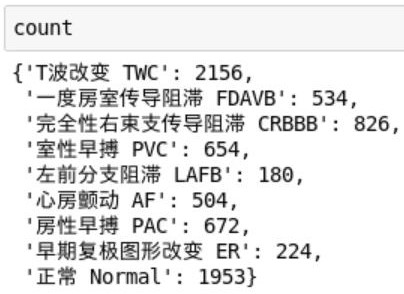
\includegraphics[width=0.65\linewidth]{img/abnormal_count.jpg}
		\caption{\label{fig:class_count} Class count of training data}
	\end{figure}
\end{center}

\subsection{Problem description}
The goal of this problem is to come up with a model using the provided 6500 training data to label an ECG that lies within the 8 categories mentioned above with all of its abnormalities, or of course normal if one has none. 

\subsection{A deeper look}
Knowing the fact that most abnormal ECG changes can co-exist, we came up with 3 different methodologies to solve this problem. 

\begin{itemize}
	\item Single-label classification problem of every possible combinations of 8 abnormalities
	\item Multi-label classification/labeling problem
	\item Multiple 2-classes classification problem
\end{itemize}

However each data entry can theoretically have 1 to 8 labels(neglecting abnormalities that are naturally contradicting), making possible class pool huge($2^8 + 1 = 257$). The provided data only has 107 different combinations and more than half of which has less than 5 data entries. Therefore treating each combination as a separate class is not wise. 

For multi-label classification, we not only have the problem of training data hardly spans half of the possibilities, the very uneven distribution of each class can also be problematic. 

Since this is a real world problem and we have been using human intelligence to solve this problem for decades, it is hard to be ignorant about the experience doctors built and the rules researchers came up with. After all, we are dealing with a tiny subset of the real problem: labeling 8 out of more than 100 ECG changes\cite{litfl}. Thus we finally used the last methodology, treating the problem as 8 two-class classification sub-problems, because we want to be able to easily meddle with our techniques for each different abnormalities so that we can add human experience and knowledge to our model.

\section{Preprocessing}
Data preprocessing is an integral step in Machine Learning as the quality of data and the useful information that can be derived from it directly affects the ability of our model to learn \cite{Dhairya}. When we as human-beings look at information around us, we subconsciously "preprocess" the information and come up with a conclusion. This is why we can read text in various fonts and easily capture objects from a very noisy picture. Our model on the other hand, have very limited ability to extract key information from data so it is tremendously important for us to preprocess our data before feeding it into our model.

\subsection{Detecting QRS complex}
There are many open source tools and algorithms available online for detecting QRS complex. It is the most important preprocessing of data in our work since we will be using ECG data of just one beat(one complete cycle of heart beat). We will also try to find R point of each beat to calculate heart rate, to determine Arrhythmia as well as roughly locating P segment, ST segment and T wave. 

Here we used the offline version of an open source toolkit on github \cite{Sznajder} as a base project and modified it to suit our need. 

First off we changed the structure of input data. The original project requires both voltage and timestamp data as inputs, however the timestamp data is actually redundant. Thus I modified it to accept 1 dimensional time series data.

Secondly I noticed the toolkit is using $butter$ and $lfilter$ method from $sklearn.signal$ module to filter out high and low frequency noise from the raw data. I think our primal goal here is to accurately find R point rather than give a nice looking ECG, so I built a slider tool to test and find out the best parameters for high and low frequency cutoff values to magnify wave features in our ECG, i.e. amplitude and slope. \textbf{todo: post a screenshot for the simple slider tool and the high, low cut of the final band-pass filter}

The tool then calculates the discrete derivative of the signal and take the square of it. At last it calculates the integral of the result to find out the steepest small interval and thus roughly find out where the QRS complex is. In other words, it is calculating the energy of the electricity of equally spaced small intervals, and in most cases if not all, the QRS complex will have way more energy than other segments of the ECG. 

After we get the integrals, aka. energy levels of the lead in the ECG, we use a peak detection method \cite{Slavic} using Pan-Tomkins algorithm \cite{Sznajder}. At this point we have a list of possible R points calculated based on "intervals of the most energy". However, due to the fact that the QRS complexes are very short and depending on how we slice those small intervals, the point we get may not lie right on R point, but on either QR segment or RS segment instead. \textbf{get a graph of result not right on R points}. 

At least we have a somehow accurate interval, i.e. we know where the QRS complexes are, just not the actual R point. This is good enough for our purpose though. We can find the maximum/minimum point of the small segments near the R points in the result (note that aVF lead is generally drew upside down) and find the minimum/maximum point before and after the previous point to get possible Q,R,S points.

The efficiency of this process is quite good. \textbf{todo: give an example of how long it takes to process a certain number of data}

\subsection{Slicing ECG based on beats}
We obtained a list of QRS complex locations(indexes) in the previous step. We still want to cut the full ECG based on pulses. Note that for each data entry, we can obtain 12 different sets of R points. Given the fact that data in 12 leads are taken simultaneously, their R points should align pretty good. Though we really only need one set to do the splitting, it is such a waste to disregard the others. What we did was to obtain R points of all 12 leads using the above mentioned technique, then find the most common length within these 12 sets of R points. For instance, if the resulting R points of 12 leads 
$$R = \begin{matrix}
23&447&902&1342&1898&2256&2712&3123&3589 \\
&449&904&1345&1897&2252&2713&3125 \\
&448&903&1344&1898&2253&2716&3124 \\
&445&900&1340&1897&2255&2714&3121 \\
&444&900&1341&1898&2254&2712&3119&3592 \\
&441&898&1338&1895&2253&2712&3120 \\
&447&902&1340&1897&2255&2714&3125 \\
&445&900&1342&1897&2255&2714 \\
&444&903&1340&1898&2258&2712&3121 \\
&445&901&1340&1895&2255&2714&3121 \\
&443&901&1342&1897&2253&2714 \\
21&445&900&1340&1897&2255&2714&3121 \\
\end{matrix}
$$

has length $length = [9, 7, 7, 7, 8, 7, 7, 6, 7, 7, 6, 8]$, we will take $l_{most\_common} = 7$ as the most common length. In reality the above matrix won't align so nicely like this, so we need to find and eliminate outliers ourselves. We take the leads with the most common length, namely the II, III, aVR, aVF, V1, V3, V4 and use the average of each column as the "golden rule". We then find the outliers by looping though all other leads and calculate the minimum difference between each R index and every R index in the golden rule. For example, in lead I, the very first R index $23$ is \textbf{not close to} any index in the golden rule, thus it is an outlier and needs to be removed. As for the ones that are shorter than the "golden rule", we find out where(which pulse) the it is missing and simply insert with the average of the "golden rule" of that pulse. Now we should have a $NUM_{pulse} \times 12$ matrix that is perfectly shaped so we simply calculates the average of each column to obtain the ultimate R point indexes of the case.

We are now able to locate where each QRS complex is, but it is still hard to accurately locate P and T wave of each pulse because many of abnormalities will result in significant changes with P and T wave. To achieve our goal efficiently, we simple split each pulse 50 points after the middle point of two continuous R indexes. Because P wave is generally shorter than ST-T segment. For example, $\begin{matrix}
[449&904]
\end{matrix}$ will have splitting points at $\lfloor \frac{449 + 904}{2} + 50\rfloor = 726$ 

This method can eliminate noises that occur in a subsets of leads assuming leads without noise still dominates the data entry. However it still has its limitation. It does not help with the case where every single lead is affected by significant noise. \textbf{For example, add the case in the testing data set with tremendous noise}

Here is a real result after applying the technique. Showing the number of pulses, i.e. the length of detected R indices of cases \textbf{where the number of pulses detected in 12 leads are not the same}. We can see that there are 34 out of the first 300 cases does not have consistent number of pulses detected, while the most common number of pulses technique works for all of them. Thus it performs relatively stable and is giving us what we need.

\begin{figure}[H]
	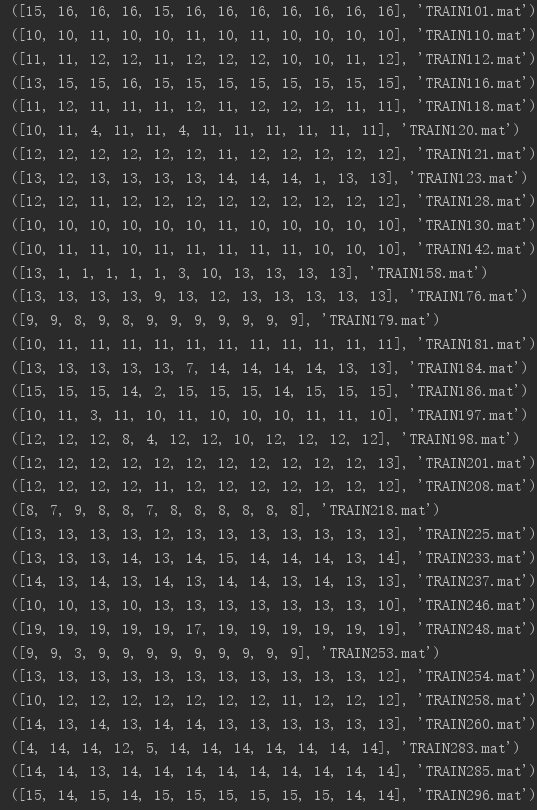
\includegraphics[width=0.8\linewidth]{img/pulse_num.png}
	\caption{\label{fig:pulse_num} Number of pulses in 12 leads}
\end{figure}

\subsection{Enriching data set}
This is yet another important technique to improve machine learning performance. Considering the labor and time cost of gathering training data, it is often not viable to gather data that can perfectly cover all possibilities of an abnormality. Human can learn how to distinguish one abnormality from another by comparing very few cases because we are very good at extracting key features from a case. However, this is comparably hard for machines. What we can do to help machines though is to create data that are different in irrelevant features while keeping the key features the same. For instance, if we were to write a program to determine whether a picture has apples in it, we only care about whether at least one apple exists, not its location, or color or orientation. Thus if we can create pictures with both green and red apples locating in every corner of the picture in various orientations, we can train a more general model to determine the existence of apples.

Here I used two basic technique to enrich or data. One is adding minor noise to the data and the other one is messing up the order of each pulse. 

After consulting with cardiologist in our team, we decide that an noise ranging $[-0.05, 0.05] mV$ won't change the key features that are deterministic. Thus in addition to original training data, we created considerable amount of data with "minor noise".

Also, for most abnormalities, the order of the pulses doesn't really hurt the diagnoses much. With the ability to split each pulse in a case, I created more data by messing up the order of pulses. For example, a data entry is originally ordered like $\overbrace{pulse_1, pulse_2, ... , pulse_10}^{10 pulses}$. We can create a number of data that looks like $\overbrace{pulse_8, pulse_2, pulse_6, ... , pulse_k}^{10 pulses}$

\section{Solving the problem}
Finally we are in business. As we mentioned in the abstract, we used a number of machine learning/deep learning techniques along with some rule-based methods to label our data. Given the fact that all abnormal wave change are different, we used different models for each abnormality based on their characteristics. However, there are two models appeared in every single cases. I would like to talk about these two first.

\subsection{Two base models}
\subsubsection{5000 Model}
As the name suggests, our input data has length 5000. In other words, we are modifying our variable length training data and make them all with the of the same length. We choose the length 5000 for the following reasons. 
\begin{itemize}
	\item Majority of data have length close to 5000
	\item We only have one label for each ECG, so 5000 is a good length to include sporadic abnormalities.
\end{itemize}
Thus we will be dealing with 3 scenarios explained below.
\begin{itemize}
	\item $length_{original} = 5000$. This is the trivial case. We simply keep it what it is.
	\item $length_{original} < 5000$. In this case we append 0s to both the start and the end of the data to forcibly make it has length of 5000.
	\item $length_{original} > 5000$. This is the tricky case. We calculate the remainder of the length divided by 5000 and see if it is less than 1000. 
	\subitem If so, we cutoff the start and the end of the data by half of the remainder to make it dividable by 5000. Then simply divided the data into $\lfloor \frac{length_{original}}{5000} \rfloor$ pieces. The first and the last one second of an ECG are often noisy anyways.
	\subitem If the remainder is greater than 1500 though, we calculate the starting indices of the split as follows
%	\begin{equation}
%	ind = \{n \cdot \frac{length-5000}{\lfloor \frac{length}{5000} \rfloor}, 0 \leq n \leq \lfloor \frac{length}{5000} \rfloor, n \in \mathbb{Z}\}
%	\end{equation}
	An simple example would be a data entry of length 22000 will have starting points at $0, 4250, 8500, 12750, 17000$, or in other words, we will slice the original data into 5 pieces with length 5000 with ranges:
	$$
	\begin{matrix}
	0&5000 \\
	4250&9250 \\
	8500&13500 \\
	12750&17750 \\
	17000&22000 \\
	\end{matrix}
	$$
\end{itemize}
Our inputs are now in the right shape. We still have concerns about the data distribution. Recall that we are building a 2 class classifier, we need to balance our data. Also note that we are not distinguishing one abnormality with only the normal ones, but every other data without that abnormality. This makes the number of negative data much more than the number of positive ones. Here we used data enrichment techniques we introduced above to populate positive data to match the size of negative data. We are not truncating negative data here because we want our model to be "familiar" with all possible cases that should not be classified positive.

Now that we have our inputs ready to roll, let's talk about the model. We mainly used $Conv1d$ layer from tensorflow based keras. The reason behind this is that our inputs are one dimensional time series. Our target features lie within the pattern of the time series. Since converting our data into images will result in most pixels being meaningless, we believe that $Conv1d$ would work as well as converting our data to images and using $Conv2d$ layers, if not better. 

In general, we used Conv1D of depth 6 followed by fully connected Dense layer of depth 4 along with a output layer. Shown below is just an example of what the model looks like. We have tried a lot of different minor modifications based on how many original data we have for the specific abnormality and how long our target feature is.
\begin{figure}[H]
	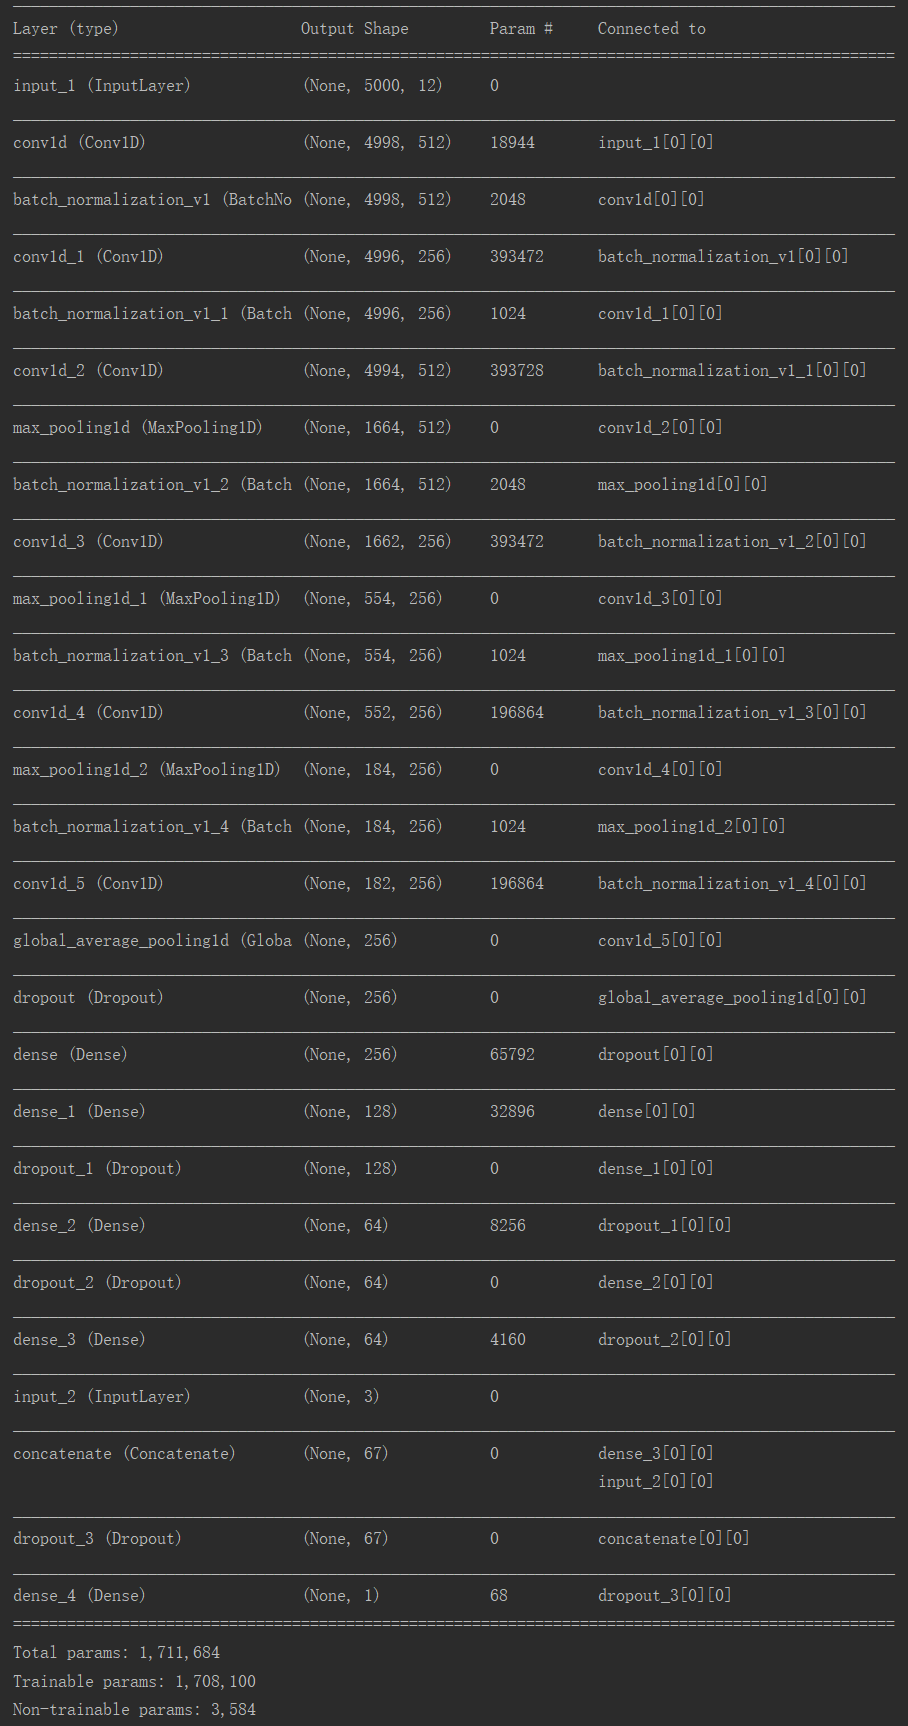
\includegraphics[width=\linewidth]{img/model_summary.png}
	\caption{\label{fig:model_summary_5000} 5000 Model Summary}
\end{figure}
We inserted normalized age and sex data into the Dense layer since there are some abnormalities that is more common in one gender/elder people and less in the opposite. 

\subsubsection{Pulse Model}
Some abnormalities, such as blocks can be found in every single pulse if one has it. We can have much more training data if we consider each pulse as a standalone data entry. Also, doing this can enable us to detect abnormalities in real time. 

Here we used pulse splitting method mentioned above to split one case into pieces consisting data of one pulse only. To make the shape of our input data looks nice, we set a fixed length of 500. Pad 0s to the shorts and truncate the longs. We do this on the start and the end of each pulse. Thus the input shape for this model is $500 \times 12$.  

Everything else besides length is pretty similar to the 5000 model above.

\subsection{Abnormality specific tuning}
\subsubsection{Atrial Fibrillation (AF)}
Atrial Fibrillation, aka. AF is "characterized by high-frequency excitation of the atrium that results in both dyssynchronous atrial contraction and irregularity of ventricular excitation"\cite{Staerk}. The most significant characteristics of AF appear on ECG is that the amplitude of its P wave is very low. Its P wave consists of mostly high frequency low amplitude "trembles" \cite{Husser}. Additionally, AF may not happen in every single pulse.
\begin{figure}[H]
	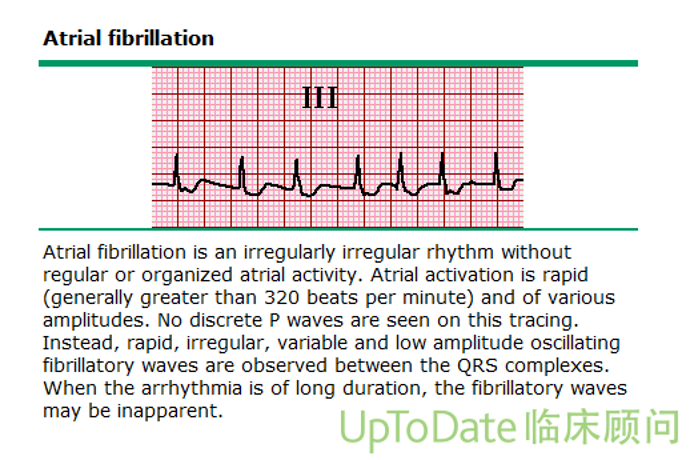
\includegraphics[width=\linewidth]{img/AF.png}
	\caption{\label{fig:AF} Atrial Fibrillation. \cite{Kumar}}
\end{figure}
With that being said, we used the 5000 model as our base model and had some minor tweaks to it since the key feature, the P segment is relatively wide. We were able to achieve more than $97\%$ 10 folds validation accuracy offline and got $0.9588\%$ testing f1 score online.

\subsubsection{First-degree Atrioventricular Block(FDAVB)}
This abnormality works pretty well with our base model so we did not make much modification or research deeper into it. The final f1 score for FDAVB is $0.9093\%$

\subsubsection{Complete Right Bundle Branch Block(CRBBB)}
\begin{figure}[H]
	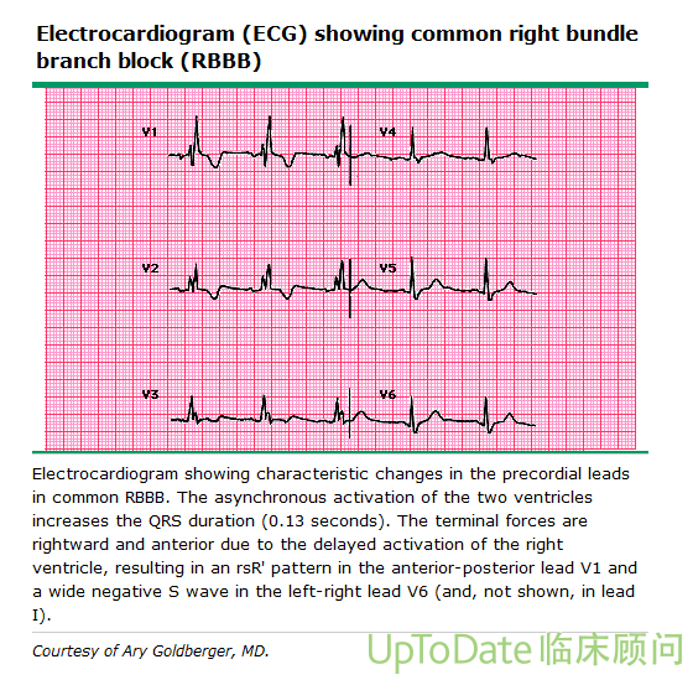
\includegraphics[width=\linewidth]{img/RBBB.png}
	\caption{\label{fig:RBBB} Complete Right Bundle Branch Block \cite{UptoDate}}
\end{figure}
CRBBB has the most obvious feature with its "M" shaped R wave. No other abnormalities have similar feature like CRBBB. This might be the easiest among this subset of abnormal ECG changes. We got surprisingly f1 score of $1$ on leader board a on our first submit with the base pulse model and final f1 score of $0.9539$ on testing data. Offline validation accuracy was more than $99\%$ 

\subsubsection{Left Anterior Fascicular Block(LAFB)}
\begin{figure}[H]
	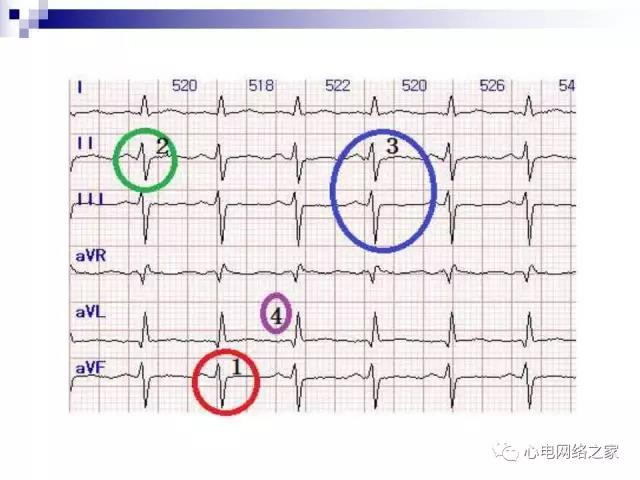
\includegraphics[width=\linewidth]{img/LAFB1.jpg}
	\caption{\label{fig:lafb1} Left Anterior Fascicular Block \cite{Yu}}
\end{figure}
LAFB is a tricky one because convolutional neural network is good at extracting "shape" features. In our case it would be "how voltage is changing". However, LAFB requires something else to be diagnosed. 
\begin{figure}[H]
	
\includegraphics[width=\linewidth]{img/LAFB2.jpg}
	\caption{\label{fig:lafb2} LAFB diagnoses \cite{Yu}}
\end{figure}
We see that the key feature here is whether the case has left axis deviation and how much. There is no way we can extract that feature solely from "shape". Thus our convolutional models is very unstable here. We came up with a toolkit to roughly calculate the axis. We also wrote a function to follow the steps shown above to diagnose LAFB with rules. The function works pretty well on training data with accuracy more than $94\%$. However, it does not work well on the 500 testing data for leader board A. My takeaway here is that we should have trust our method more since 500 is relatively small data set to judge a multi-labeling problem with 9 classes. Our final approach is to use all the tools we had, both the 5000 model and the pulse model, along with the rule-based function we wrote to obtain 3 predictions for each case. Then take the vote of these 3 predictions as our final answer. We set that if 2 models out of 3 votes 1, then we label the case with LAFB. 

Further thoughts after the contest is that we could have played with the weights instead of prediction to do the vote. We also should have manipulated the weights of each model. Simply put, we should have trained a mini-model for our voting instead of simply counting the positive predictions. 

Our offline accuracy for LAFB was above $90\%$ and f1 score for leader board based on 500 testing data was $0.895$. Sadly the final f1 score dropped a lot to $0.71$. I think this has much to do with our voting system. 

\subsubsection{Premature Ventricular Contraction(PVC)}
\begin{figure}[H]
	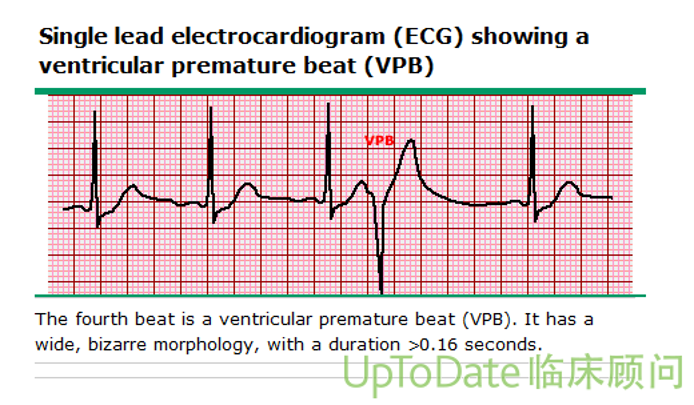
\includegraphics[width=\linewidth]{img/PVC.png}
	\caption{\label{fig:PVC} Premature Ventricular Contraction \cite{UptoDate}}
\end{figure}
PVC is also sporadic so the pulse model is not well suited. Luckily the characteristics of PVC is very obvious. We used the based model but with shorter width and larger kernel size and achieve about $95\%$ offline validation accuracy. F1 score of the 500 testing data is $0.922$ and the final f1 score is $0.92$.

\subsubsection{Premature Atrial Contraction(PAC)}
\begin{figure}[H]
	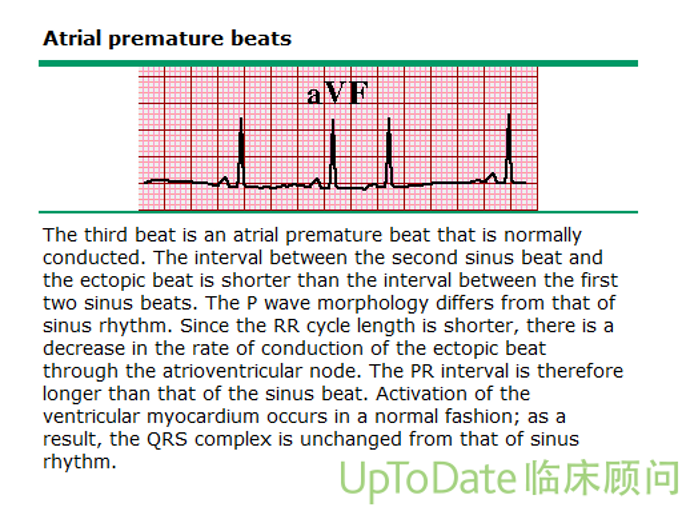
\includegraphics[width=\linewidth]{img/PAC.png}
	\caption{\label{fig:PAC} Premature Atrial Contraction \cite{UptoDate}}
\end{figure}
This is another naughty abnormality. It was pretty hard for us to improve at around $80\%$ accuracy. The diagnosis of PAC highly relies on heart rate and how its heart rate is irregular. Therefore we calculated more parameters and inserted them into our Dense layers and hoping it would help. We calculated the standard deviation of heart rate, and the maximum difference between RR intervals. 
It is a pity that we did not realize we can put PAC and AF in one model since they logically do not co-exist. 
We got approximately $85$ validation accuracy offline and f1 score of $0.8$ on the 500 testing data. The final f1 score dropped a little to $0.7863$.

\subsubsection{Early Repolarization(ER)}
\begin{figure}[H]
	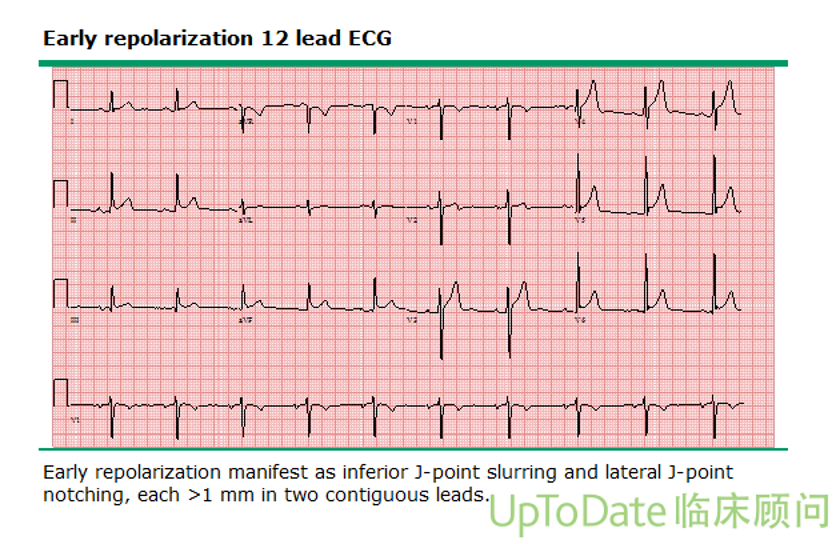
\includegraphics[width=\linewidth]{img/ER.png}
	\caption{\label{fig:ER} Early Repolarization \cite{UptoDate}}
\end{figure}

\subsubsection{T Wave Change(TWC)}
TWC did not seem to be harder than others. Its characteristics are obvious. T wave is wide and the changes are often significant.
\begin{figure}[H]
	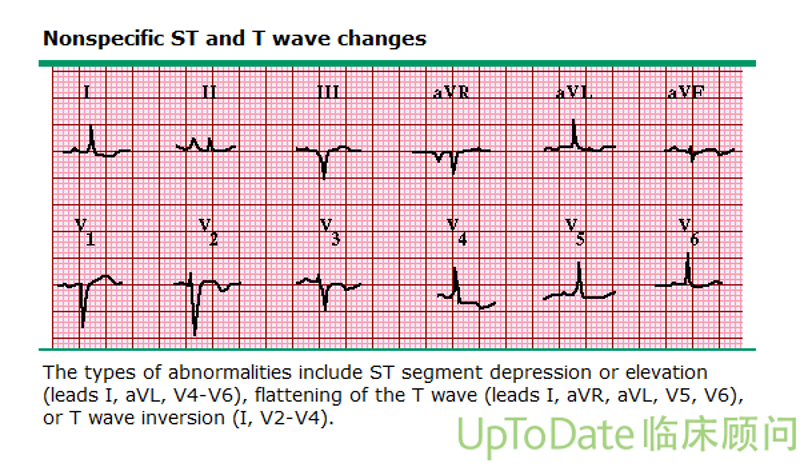
\includegraphics[width=\linewidth]{img/twc.png}
	\caption{\label{fig:twc} T Wave Change \cite{UptoDate}}
\end{figure}
We used our based model and achieved more than $90\%$ offline validation accuracy. The f1 score for the 500 testing data was $0.882$. However, the final score dropped drastically to $0.7287$. After some deeper research, we found that one possible reason why our f1 score dropped a lot is that TWC has a number of sub-categories, as shown below.
\begin{figure}[H]
	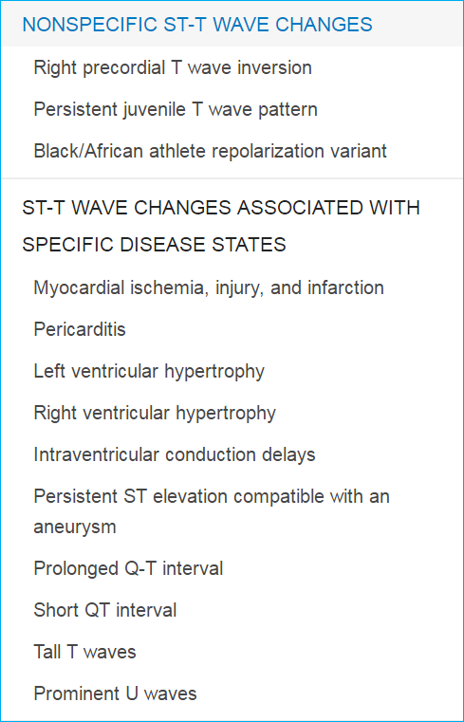
\includegraphics[width=\linewidth]{img/twc2.png}
	\caption{\label{fig:twc2} TWC in details \cite{UptoDate}}
\end{figure}
We think our training data did not span every single one of these changes or did not distribute evenly. Also it is hard to say that our validation data was good enough to show how our model perform for the same reasons. In practice, I think we should split TWC into more specific abnormalities to get more accurate models.

%\begin{acknowledgments}
%	We wish to acknowledge the support of Tsinghua University and every organization who made this contest possible. It is a great opportunity for a rookie like me to get my hands dirty on ECG data and to  learn so much along the way. I only have weeks of experience and knowledge in ECG but I found this a tremendous valuable field. I hope to see machines can free doctors from tediously reading tons of ECGs and contribute more to innovative stuff that machines are not capable of.
%\end{acknowledgments}

\appendix

\section{Practicing doctors per 1000 population}

\begin{figure}[H]
	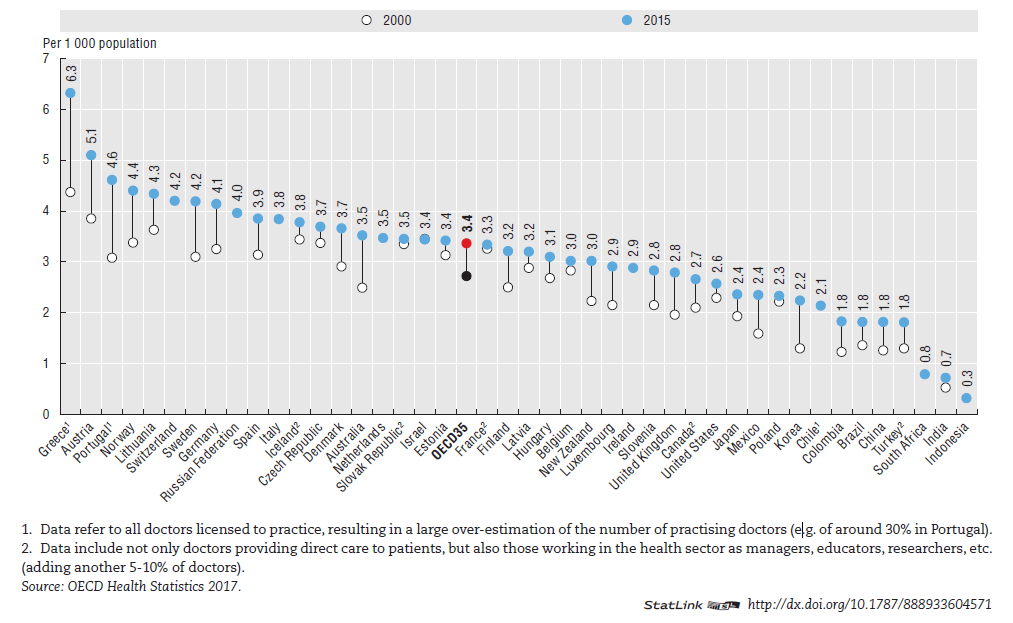
\includegraphics[width=\linewidth]{img/doc_per_1000.png}
	\caption{\label{fig:doc_per_1000} Practicing doctors per 1000 population in 2000 and 2015. \cite{OECD}}
\end{figure}

\section{Scoring Rubrics}
First of all, define 4 parameters for abnormality $j$, where $0 \leq j \leq 8$
\begin{equation}
TP_j = |\{x_i|y_j \in Y_i, y_j \in f(x_i), 1 \leq i \leq N\}|
\end{equation}

\begin{equation}
FP_j = |\{x_i|y_j \notin Y_i, y_j \in f(x_i), 1 \leq i \leq N\}|
\end{equation}

\begin{equation}
TN_j = |\{x_i|y_j \notin Y_i, y_j \notin f(x_i), 1 \leq i \leq N\}|
\end{equation}

\begin{equation}
FN_j = |\{x_i|y_j \in Y_i, y_j \notin f(x_i), 1 \leq i \leq N\}|
\end{equation}
Then calculate $precision$, $recall$ and $F_1$ score

\begin{equation}
Precision_j = \frac{TP_j}{TP_j + FP_j}
\end{equation}

\begin{equation}
Recall_j = \frac{TP_j}{TP_j + FN_j}
\end{equation}

\begin{equation}
F_{1j} = \frac{2 \cdot Precision_j \cdot Recall_j}{Precision_j + Recall_j}
\end{equation}
Finally calculate the average $F_1$ score of all 9 classes.
\begin{equation}
F_1 = \frac{1}{9} \sum F_1j
\end{equation}
%
% ---- Bibliography ----
%
% BibTeX users should specify bibliography style 'splncs04'.
% References will then be sorted and formatted in the correct style.
%
% \bibliographystyle{splncs04}
% \bibliography{mybibliography}
%
\bibliography{bib_ecg_}
\end{document}
